\documentclass[9pt]{osa-supplemental-document}

\setboolean{shortarticle}{false}

\title{Characterising measurements of vessel diameter in optical coherence tomography angiography and correcting underestimations caused by shear-induced artefacts: supplemental document}

\author{} % leave blank: author information is added during production

\begin{abstract}
This document shows the manually annotated ground truth vessel boundary compared against the cross-sectional optical coherence tomography angiography (OCTA) signal during the different phases of the contrast passage.
\end{abstract}

\setboolean{displaycopyright}{false}

\begin{document}

\maketitle

\section{Ground truth vessel boundaries across the contrast passage}

Vessel boundaries for the ground truth diameter were manually annotated from individual frames of the OCTA time stack and confirmed against adjacent frames. For characterisation and calibration, frames were selected from the peak of the bolus passage due to higher contrast. Figure~\ref{fig:phases} shows that the horizontal and vertical boundaries annotated at peak contrast remained in good agreement with the vessel cross-section as it appears in the post-bolus phase.  In the pre-contrast phase, the vertical boundaries are in agreement, but the shear-induced hourglass artefact reduces the OCTA signal significantly at the lateral edges of the vessel leading to an underestimation of vessel width.

\begin{figure}[htbp]
\centering
\begin{minipage}[t]{0.32\linewidth}\centering\textsf{\textbf{Pre}}\\[2pt]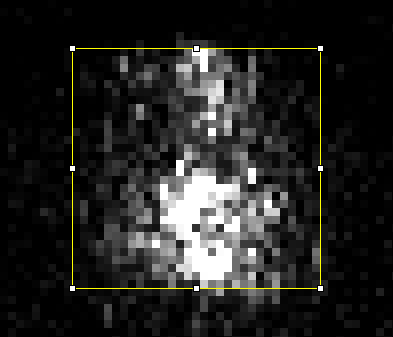
\includegraphics[width=\linewidth]{figures/supp_phase_pre.png}\end{minipage}\hfill
\begin{minipage}[t]{0.32\linewidth}\centering\textsf{\textbf{Peak}}\\[2pt]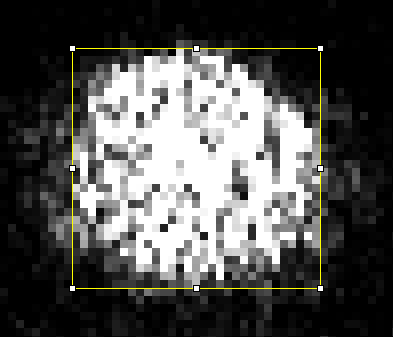
\includegraphics[width=\linewidth]{figures/supp_phase_peak.png}\end{minipage}\hfill
\begin{minipage}[t]{0.32\linewidth}\centering\textsf{\textbf{Post}}\\[2pt]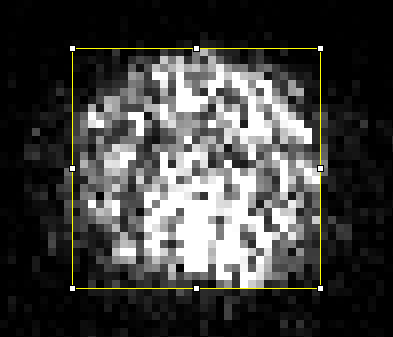
\includegraphics[width=\linewidth]{figures/supp_phase_post.png}\end{minipage}
\caption{Individual frames of a DyC-OCT angiogram timecourse of the same vessel cross-section at pre-contrast, peak-contrast and post-contrast phases. Vessel boundaries were annoted manually during the peak contrast phase using ImageJ (Fiji distribution), shown as yellow boxes here. Note that the boxes shown in each frame are identical in size and positioning and based only on the segmentation of the vessel during the peak contrast phase.  All panels use the same dynamic range.}
\label{fig:phases}
\end{figure}

\end{document}
